\input{commun/presentations.tex}
\input{03-Meteo/img/barometreTorricelli.tex}
\input{commun/echelleAltitudeMetres.tex}

\title[Séance 5 - Atmosphère]{Séance 5 \\ Atmosphère}

\begin{document}
 \begin{frame}
 \titlepage
 \end{frame}
 
 \begin{frame}
 \tableofcontents
 \end{frame}
 
 \section{L'atmosphère}
	\begin{frame}{L'atmosphère}
	
	\question{Qu'est-ce que l'atmosphère ?}
	\pause
	\question{De quoi est composée l'atmosphère terrestre ?}
	\end{frame}	 
	
	
	\begin{frame}{Aéroport}
	\begin{columns}
		\begin{column}{0.52\textwidth}
		\begin{figure}[H]
			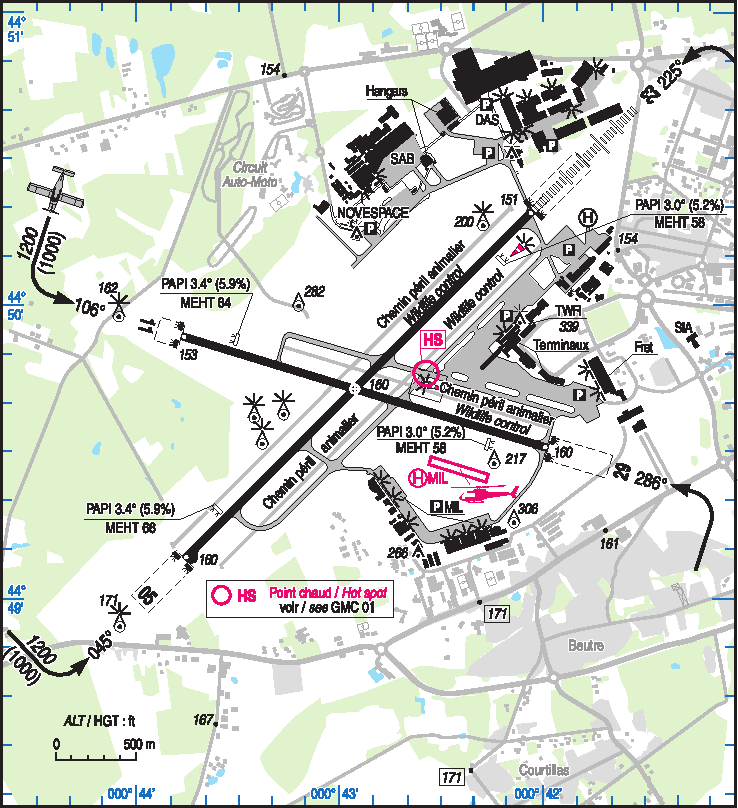
\includegraphics[width=0.95\linewidth]{02-Navigation/img/vacLfbd.pdf}
			\legende{Extrait de la carte VAC de Bordeaux LFBD}{img:vacLfbd}
		\end{figure}	
		\end{column}
		\begin{column}{0.48\textwidth}
			\begin{itemize}
				\item Les pistes sont nommées selon les dizaines de leur orientation magnétique
				\item Le numéro d'une piste et de la piste opposée ont toujours un écart de 18 (= 180\textdegree )
			\end{itemize}
		\end{column}
	\end{columns}
	\end{frame}
	
	\begin{frame}{Aéroport}
	\begin{columns}
		\begin{column}{0.55\textwidth}
			\begin{itemize}
				\item Si un aéroport a plusieurs pistes parallèles, on les nomme suffixe avec leur position gauche (L, left), droite (R, right), et s'il y en 3, centre (C, center)
			\end{itemize}
		\end{column}
 		\begin{column}{0.45\textwidth}
 		\begin{figure}[H]
			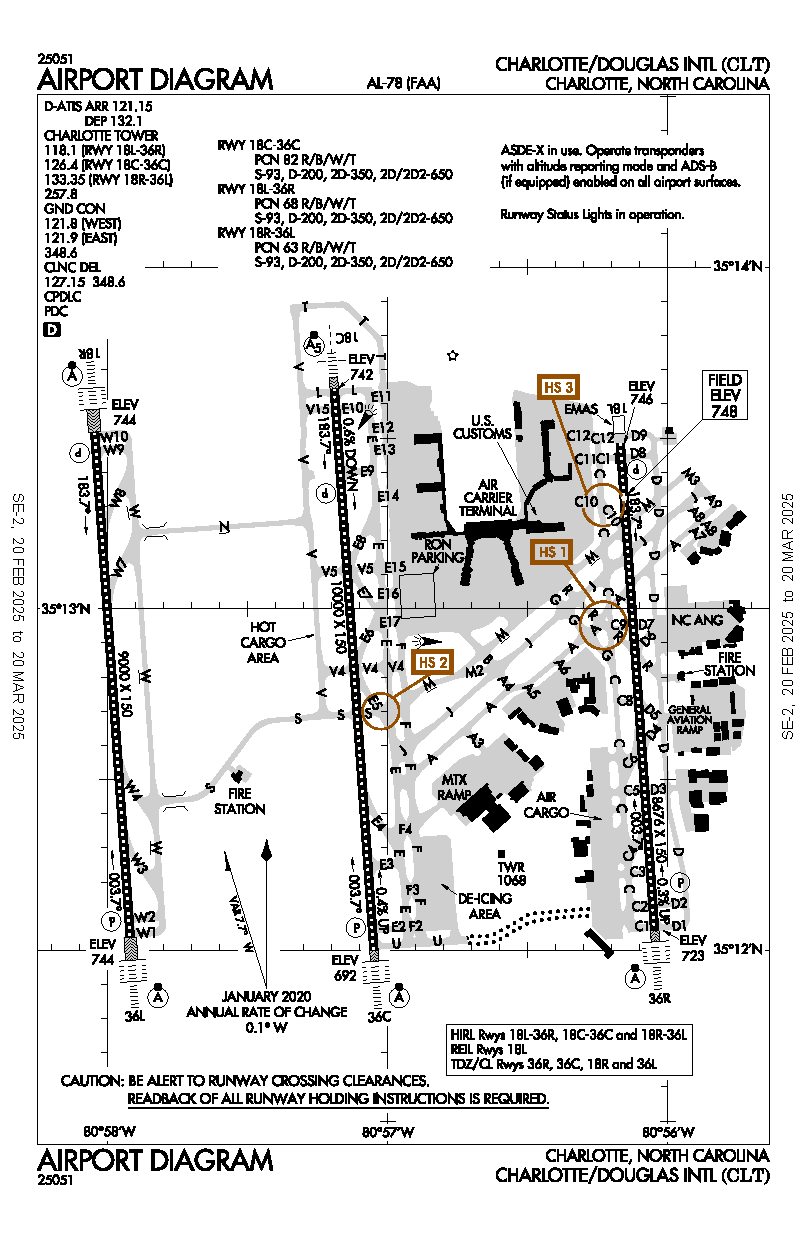
\includegraphics[width=0.8\linewidth]{02-Navigation/img/kcltAirportDiagram.pdf}
			\legende{Schéma de l'aéroport de Charlotte KCLT}{img:kcltAirportDiagram}
		\end{figure}	
		\end{column}
	\end{columns}
	\end{frame}	
	
 
 	\begin{frame}{Tour de piste}
	\begin{figure}[H]
			\centering
			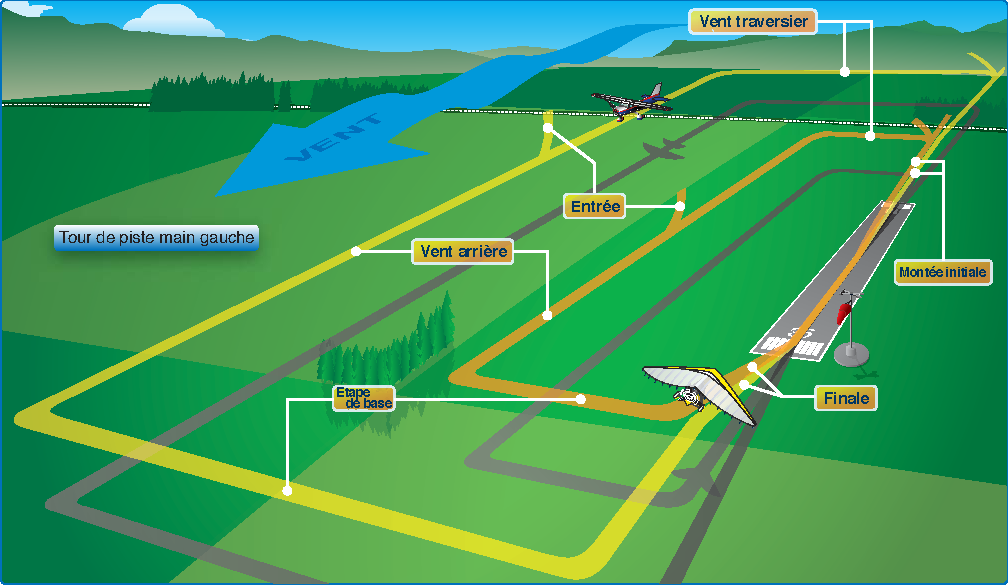
\includegraphics[width=0.9\linewidth]{02-Navigation/img/tourDePiste.pdf}
			\legende{Schéma d'un tour de piste}{img:tourDePiste}
		\end{figure}	
	\end{frame}	
\appendix 
\section{QCM}
\qmcBia{Navigation, réglementation, sécurité des vols}
{2}{Comment sera numérotée une piste d'orientation magnétique de 104\textdegree}
{11}
{10}
{04}
{104} 
{}

\qmcBia{Navigation, réglementation, sécurité des vols}
{3}{Que permet d'indiquer la manche à air sur un aérodrome ?}
{le numéro de la piste en service}
{la température de l'air}
{le sens et la vitesse du vent}
{le sens d'atterrissage, dos au vent} 
{}

\qmcBia{Navigation, réglementation, sécurité des vols}
{3}{Quelle est la position d'un avion qui vole en circuit de piste parallèlement à la piste ?}
{étape de base}
{vent debout}
{vent arrière}
{vent de travers} 
{}

\qmcBia{Navigation, réglementation, sécurité des vols}
{3}{Sur tous les aérodromes ouverts à la circulation aérienne publique (CAP), la réglementation impose la présence : }
{du numéro de la piste en service sur la tour de contrôle}
{d'un hangar pour héberger les avions de passage}
{d'une manche à air}
{d'un T indiquant la piste en service} 
{}

\qmcBia{Navigation, réglementation, sécurité des vols}
{4}{Un tour de piste main gauche signifie : }
{que l'avion doit se poser sur la partie gauche de la piste}
{que le pilote doit piloter avec la main gauche pour des raisons de sécurité}
{que la manche à air est à gauche de la piste} 
{que le pilote effectue le dernier virage avec la piste à sa gauche}
{}
 
\input{commun/beamerSlidesBiblio.tex} 
 
\end{document}
